\begin{figure*}[!htbp]
\begin{minipage}{6in}
\begin{center}

\begin{minipage}{\linewidth}
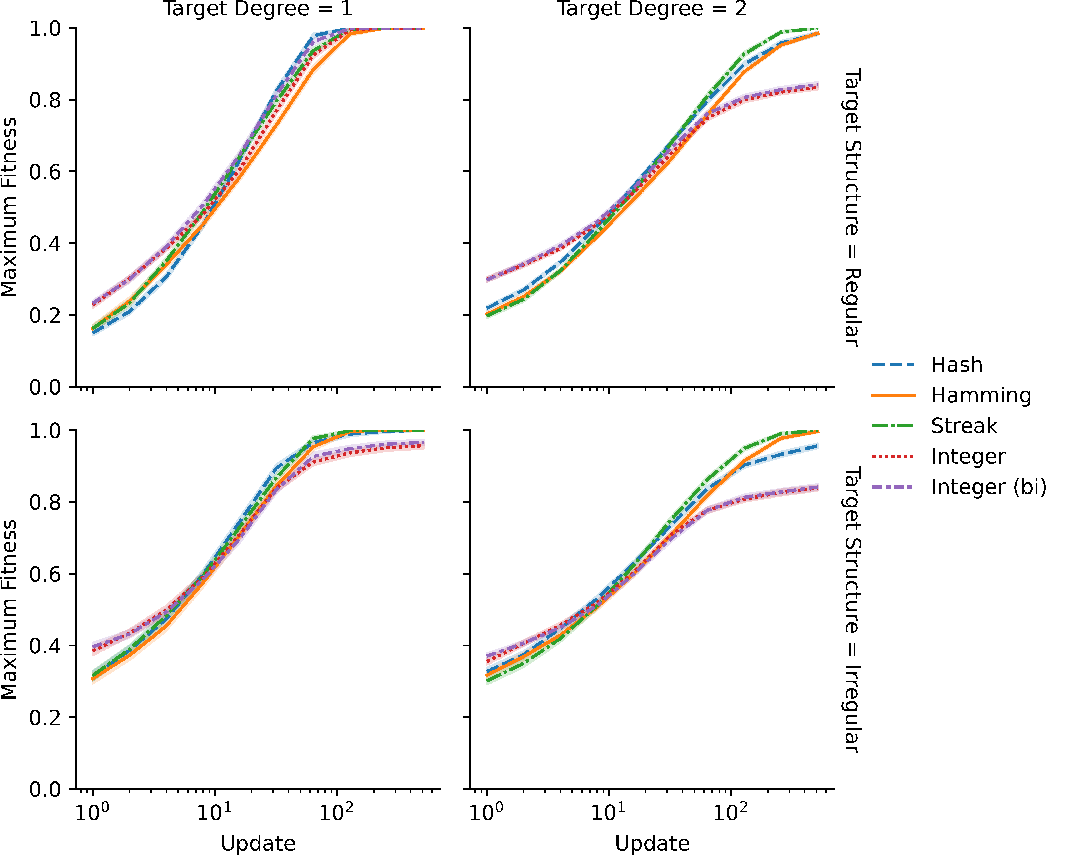
\includegraphics[width=\linewidth]{img/target_evolve_zeroinit/viz=max-fitness-line+_data_hathash_hash=c89e27249186c6a7+_script_fullcat_hash=d2023baeff76b578+ext=}
\end{minipage}
\begin{minipage}{\linewidth}
\caption{
Trajectories of adaptive evolution for each tag-matching metric on the 32-vertex graph-matching task with identically-initialized initial genomes.
Maximum fitness is the best fitness value for any individual within a population.
Reported results use each metric's best-performing per-bit mutation rate.
(See Supplementary Figure \ref{fig:evolve_zeroinit_mutsweep} for survey of how mutation rate affects adaptive evolution under each metric.)
Note logarithmic $x$-axes.
Shaded area represents bootstrapped 95\% confidence intervals across 100 replicate observations.
}
\label{fig:evolve_bests_zeroinit}
\end{minipage}
\end{center}
\end{minipage}
\end{figure*}
